% Define document class
\documentclass[twocolumn]{aastex631}
\usepackage{showyourwork}
\usepackage{bbold}

% Begin!
\begin{document}

% Title
\title{Polka-dotted Stars: Mapping the Surface of HAT-P-11}

% Author list
\author{Sabina Sagynbayeva}

% Abstract with filler text
\begin{abstract}
   
\end{abstract}

% Main body with filler text
\section{Introduction}
\label{sec:intro}

%
\section{The Data}
The data is collected by the \emph{Kepler} mission and we extracted it using
\texttt{lightkurve}, a Python package for Kepler and TESS data analysis \citep{lightkurve}.
%
\begin{figure}[ht!]
    \script{TransitFitsWithStarry.py}
    \begin{centering}
        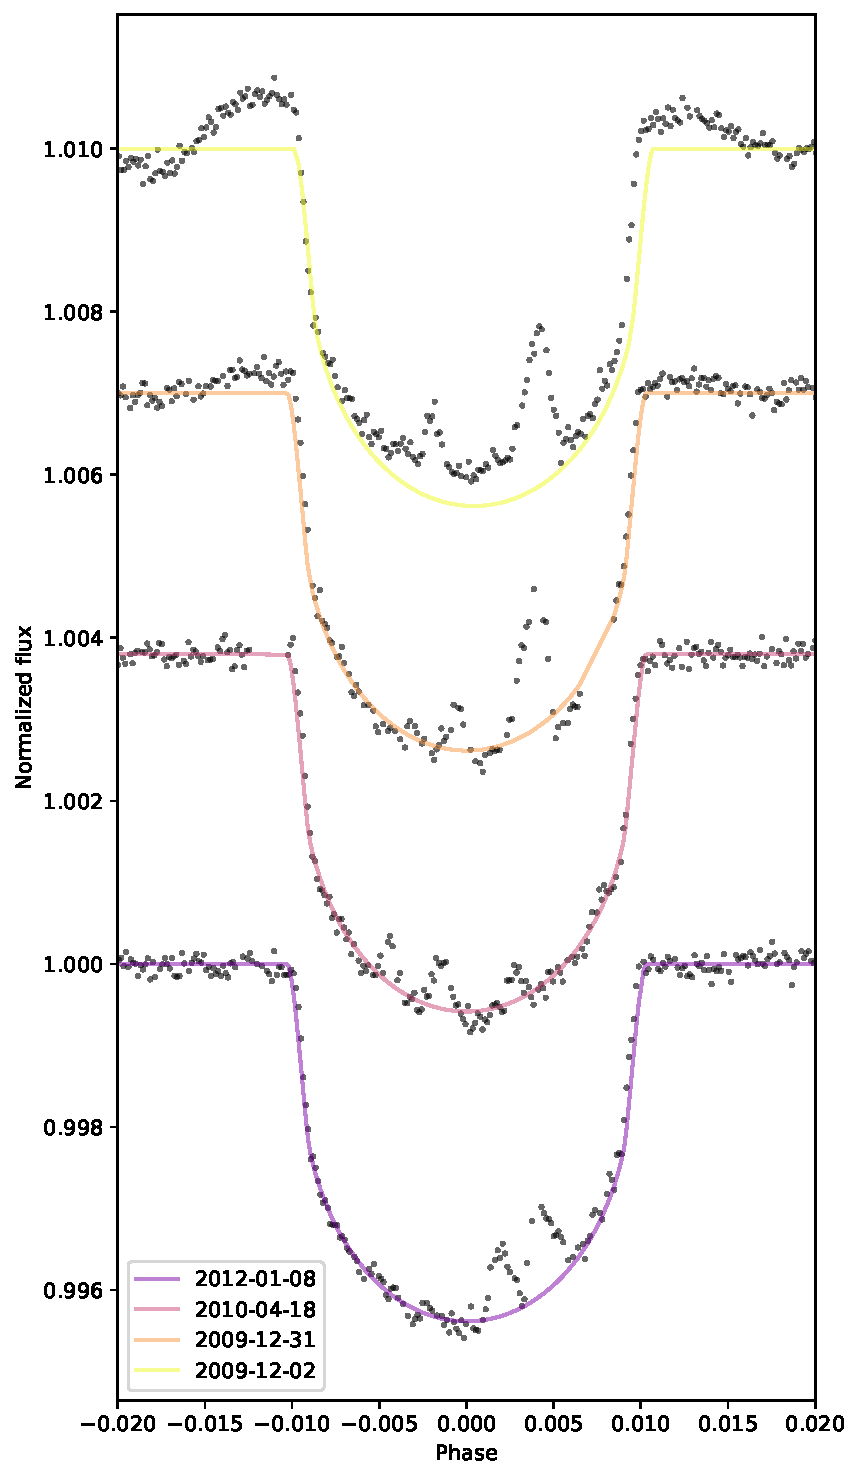
\includegraphics[width=\linewidth]{figures/TransitFitsWithStarry.pdf}
        \caption{
            Transit fits with starry -- no GPs.
        }
        \label{fig:TransitFitsStarry}
    \end{centering}
\end{figure}
%
\section{Hierarchical Bayesian model}

%
\subsection{The Model}
In this section, we will describe our Gaussian Process (GP) model and the likelihood calculation process used to estimate the model parameters. 

We solve for a large set of parameters that includes the GP hyperparameters, the star's and the planet's orbital parameters, respectively. 
\begin{linenomath}\begin{align}
    \label{eq:largetheta}
    \pmb{\Theta}
     & =
    \left(
    \theta_\bullet
    \,\,\,
    \theta_\star
    \,\,\,
    \theta_p
    \right)^\top
    \quad,
\end{align}\end{linenomath}

Separately, these parameters are defined as 
\begin{linenomath}\begin{align}
    \label{eq:thetastar}
    \pmb{\theta_\star}
     & =
    \left(
    i_\star
    \,\,\,
    m_\star
    \,\,\,
    u_1
    \,\,\,
    u_2
    \,\,\,
    P_\star
    \right)^\top
    \quad,
\end{align}\end{linenomath}
where $i_\star$ is the star's orbital inclination, $m_\star$ is the stellar mass in the units of the solar mass, $u_1$ and $u_2$ are limb-darkening coefficients,
and $P_\star$ is the rotational period of the star.

\begin{linenomath}\begin{align}
    \label{eq:thetap}
    \pmb{\theta_p}
     & =
    \left(
    i_p
    \,\,\,
    e
    \,\,\,
    \psi
    \,\,\,
    \omega
    \,\,\,
    P
    \,\,\,
    t_0
    \,\,\,
    R_p/R_\star
    \right)^\top
    \quad,
\end{align}\end{linenomath}
where $i_p$ is the planet's orbital inclination, $e$ is its eccenticity, $\psi$ is the stellar obliquity, $\omega$ is the argument of pericenter of the planet,
$P$ is the rotational period of the planet, $t_0$ is the transit start time, and $R_p/R_\star$ is the planet to star radius ratio.

We represent the GP hyperparameters as \emph{physically interesting} set of parameters $\pmb{\theta}_\bullet$ \citep{Luger2021}:
%
\begin{linenomath}\begin{align}
        \label{eq:thetaspot}
        \pmb{\theta}_\bullet
         & =
        \left(
        n
        \,\,\,
        c
        \,\,\,
        \mu_\phi
        \,\,\,
        \sigma_\phi
        \,\,\,
        r
        \right)^\top
        \quad,
    \end{align}\end{linenomath}
%
where $n$ is the number of starspots, $c$ is their contrast (defined as the intensity difference between the spot and the 
background intensity, as a fraction of the background intensity),
$\mu_\phi$ and $\sigma_\phi$ are the mode and standard deviation
of the spot latitude distribution, respectively, and $r$ is the radius
of the spots.

We assume that the prior over $\mathbb{f}_{true}$ follows a multivariate Gaussian distribution, with a mean vector of zeros and a covariance 
matrix $\pmb{\Sigma}$. We use the quasi-periodic kernel to define the covariance matrix $\pmb{\Sigma}$, which is defined by \texttt{StarryProcess}.
We assume that the observations $\mathbb{f}_{obs}$ are corrupted by additive Gaussian noise, such that:
\begin{equation}
    \mathbb{f}_{obs} = \mathbb{f}_{true} + \epsilon
\end{equation}

where $\epsilon \sim \mathcal{N}(0, \sigma_n^2)$ is the noise term. Given the GP prior and the likelihood function, we can 
calculate the joint posterior distribution over the hyperparameters $\Theta$ and the true function $\mathbb{f}_{true}$ given the observed data $\mathbb{f}_{obs}$:
%
\begin{equation}
    p(\Theta, \mathbb{f}_{true} \mid \mathbb{f}_{obs}) \propto p(\Theta) p(\mathbb{f}_{true} \mid \Theta) p(\mathbb{f}_{obs} \mid \mathbb{f}_{true})
\end{equation}
%
where $P(\Theta)$ is the prior distribution over the hyperparameters, $P(\mathbb{f}_{true} \mid \Theta)$ is the likelihood of the true function given 
the hyperparameters, and $P(f_{obs} \mid f_{true})$ is the likelihood of the observed data given the true function.
We calculate the log-likelihood function, given by:
%
\begin{linenomath}\begin{align}
    \label{eq:log-likeSabina}
    \ln p(\mathbb{f}_{obs} \mid \pmb{\Theta}) 
    =
    & -\frac{1}{2} (\mathbb{f}_{obs} - \pmb{\mu})^T \pmb{\Sigma}^{-1} (\mathbb{f}_{obs} - \pmb{\mu}) 
    \nonumber       \\[0.75em]
    & -
    \frac{1}{2} \ln |\pmb{\Sigma}| - \frac{n}{2} \ln (2\pi)
    \quad,
\end{align}\end{linenomath}
%
or, as defined in eq. 14 of \citep{Luger2021}:
%
\begin{linenomath}\begin{align}
    \label{eq:log-likeRodrigo}
    \ln \mathcal{L}_m\left(\Theta\right)
    =
     & -\frac{1}{2}
    \mathbf{r}_m^\top\left(\Theta\right)
    \big[
        \pmb{\Sigma}\left(\Theta\right)
        \big]^{-1}
    \mathbf{r}_m\left(\Theta\right)
    \nonumber       \\[0.75em]
     & -
    \frac{1}{2}
    \ln \Big|
    \pmb{\Sigma}\left(\Theta\right)
    \Big|
    -
    \frac{K}{2}
    \ln \left( 2 \pi \right)
    \quad,
\end{align}\end{linenomath}
%
where
%
\begin{linenomath}\begin{align}
        \mathbf{r}_m\left(\pmb{\Theta}\right)
         & \equiv
        \mathbf{f}_m - \pmb{\mu}\left(\pmb{\Theta}\right)
    \end{align}\end{linenomath}
%
is defined as the residual vector,
%
$\Sigma$ is the full covariance, which is defined as 
%
\begin{linenomath}\begin{align}
    \pmb{\Sigma}\left(\Theta\right)
     & \equiv
    \pmb{\Sigma_y} + \pmb{\Sigma_d}
\end{align}\end{linenomath}
%
where $\pmb{\Sigma_y}$ is the covariance of the distribution over spherical harmonic coefficient
vectors $\mathbb{y}$, and $\pmb{\Sigma_d}$ is the data covariance, which is a diagonal
matrix whose entries are the squared uncertainty $\sigma_m^2$ corresponding to each data point in the light curve.
$| \cdots |$ denotes the determinant, and $K$ is the number of data points in
each light curve.%

For faster calculations we rewrite the likelihood function using \emph{the matrix conversion lemma}, also known as 
Woodbury-Sherman-Morrison identity (see e.g. \cite{Hogg2020}).


\section{Experiments}
In this section, we describe the experiments we did on synthetic light curves before going ahead and modeling the real data. The synthetic light curves were 
generated by initializing a planet and a star of similar parameters as HAT-P-11 b and HAT-P-11 have using \texttt{starry}. Then we draw \texttt{StarryProcess} 
samples from a prior to get spherical harmonic coefficients and consequently the simulated flux. 

\subsection{Normalization of light curves}
Before going on discussing the experiments prduced for this paper, we first need to remind the reader of a subtlety of the flux normalization when we are given
the raw light curves from telescopes. The problem and the ways to tackle it were described in \cite{Luger2021a} and \cite{Luger2021b}. 

Briefly, the problem of normalization of light curves is related to the fact that the observed flux from a star can vary due to a variety of factors 
such as atmospheric effects, instrumental noise, and changes in the intrinsic brightness of the star itself. These variations can make it difficult 
to compare light curves of different stars or even the same star observed at different times. To address this problem, astronomers typically normalize 
light curves by dividing the observed flux by some factor (the median or mean of the flux) that is assumed to be constant over time. 
However, as was described in \cite{Luger2021a}, if a star has a single large equatorial spot of contrast $c$ viewed at some high inclination 
(\cite{Luger2021a} used the value of $60^o$), and the another star with a spot at the same location but with half the contrast \emph{and} a large polar spot of 
comparable contrast, then the light curves for both of the stars become indistiguishable in the relative units astronomers observe them.

In our experiments, we explicitly solve for the normalization factor and, same as other parameters, divide the modeled light curve, $\mathbb{f}_{true}$,
by a random value drawn from a sample of a posterior distribution.


\subsection{Short light curve}
\subsection{Long light curves (multiple transits)}
\section{Results and Discussion}

\bibliography{bib}

\end{document}
